% ======================================================================
% BLOQUE 3 — El Observatorio Pierre Auger
% ======================================================================
\section{Observatorio Pierre Auger}
\bloque{PIERRE AUGER}

% ---------------------------------------------------------------- 24
\begin{frame}[plain]
  \fondo[0.05]{externas/auger_tanque_escala.jpg}
  \velo[0.85]{l}
  \begin{tikzpicture}[remember picture, overlay]
    \node[anchor=north west, text=white, align=left, text width=6.2cm]
      at ([xshift=0.7cm, yshift=-0.8cm]current page.north west) {%
      {\Large\bfseries ¿Cómo se mide algo que llega una vez por km$^2$ por siglo?}\\[4pt]
      {\footnotesize (por encima de $\sim5\times10^{19}$\,eV)}\\[8pt]
      {\large $N = J\cdot A\cdot\Omega\cdot T$}\\[10pt]
      {\small Con $A\approx3000$\,km$^2$ ---unas 15 veces la Ciudad de
      Buenos Aires---, funcionando día y noche desde 2004.}\\[6pt]
      {\small Resultado: $\approx$50.000 eventos por encima de 8\,EeV en 19 años.}};
    \node[anchor=south west, text=white!85, font=\scriptsize, text width=6cm]
      at ([xshift=0.7cm, yshift=0.45cm]current page.south west)
      {Una estación del detector de superficie en la Pampa Amarilla, Malargüe};
  \end{tikzpicture}
  \creditoblanco{Foto: T.~Schulz, CC BY-SA 4.0 (Wikimedia Commons) \quad Estadística: Auger, ICRC 2025}
\end{frame}

% ---------------------------------------------------------------- 25
\begin{frame}{Una partícula con la energía de una pelota de béisbol}
  \begin{columns}[c,onlytextwidth]
    \column{0.57\textwidth}
      \centering
      \begin{tikzpicture}[x=0.56cm, y=0.8cm]
        \draw[itedaGray, thick, -{Stealth}] (9,0) -- (21.4,0);
        \node[font=\scriptsize, text=itedaGray, anchor=north] at (15,-0.4) {energía [eV]};
        \foreach \x in {9,11,...,21}{\draw[itedaGray] (\x,-0.08) -- (\x,0.08)
          node[below=3pt, font=\tiny, text=itedaGray] {$10^{\x}$};}
        \tikzset{marca/.style={thick, -{Stealth}}}
        \draw[marca, itedaTeal, very thick] (12.83,1.5) -- (12.83,0.12);
        \node[font=\small\bfseries, text=itedaTeal, align=center, anchor=south] at (12.83,1.5)
          {protón del LHC\\6,8\,TeV};
        \draw[marca, itedaOrange, very thick] (20,1.5) -- (20,0.12);
        \node[font=\small\bfseries, text=itedaOrange, align=center, anchor=south] at (20,1.5)
          {rayo cósmico\\$10^{20}$\,eV};
        \draw[decorate, decoration={brace, amplitude=6pt, mirror}, thick, itedaTealDark]
          (12.83,-0.95) -- (20,-0.95);
        \node[font=\small\bfseries, text=itedaTealDark, anchor=north] at (16.4,-1.15)
          {$\times\,10^{7}$: siete órdenes de magnitud};
      \end{tikzpicture}\\[4pt]
      \begin{minipage}[c]{0.3\linewidth}
        \centering
        \begin{tikzpicture}[scale=0.68]
          \fill[noche, rounded corners=3pt] (-1.75,-1.75) rectangle (1.75,1.75);
          \draw[white!70, thin] (0,0) circle (1.45);
          \fill[white!80] (1.45,0) circle (1.5pt);
          \node[font=\tiny, text=white!80] at (0,1.25) {Mercurio};
          \draw[itedaOrange, very thick, dashed] (0,0) circle (1.0);
          \shade[ball color=yellow!80!orange] (0,0) circle (0.14);
          \node[font=\tiny\bfseries, text=itedaOrange] at (0,-0.55) {«LHC»};
        \end{tikzpicture}
      \end{minipage}\hfill
      \begin{minipage}[c]{0.67\linewidth}
        \footnotesize\raggedright
        ¿Un LHC para $10^{20}$\,eV? Con los mismos imanes (8\,T), su radio
        sería de \textbf{$\sim$40 millones de km}: casi la \textbf{órbita de
        Mercurio}.
      \end{minipage}
    \column{0.40\textwidth}
      \begin{clave}
        \large
        $10^{20}$\,eV $\approx$ \textbf{16\,J}\\[6pt]
        \normalsize
        Una pelota de béisbol (145\,g) a 90\,km/h tiene \textbf{45\,J}.\\[6pt]
        El récord, Fly's Eye (1991): $3{,}2\times10^{20}$\,eV $\approx$
        \textbf{51\,J}.\\[6pt]
        La energía de una pelota rápida, \textbf{en un solo núcleo}.
      \end{clave}
      \vspace{4pt}
      {\scriptsize\color{itedaGray} En el centro de masa, el choque con un
      núcleo del aire equivale a «sólo» $\sim$30 LHC.}
  \end{columns}
\end{frame}

% ---------------------------------------------------------------- 26
\begin{frame}{El Observatorio Pierre Auger, en Malargüe}
  \begin{columns}[c,onlytextwidth]
    \column{0.40\textwidth}
      \centering
      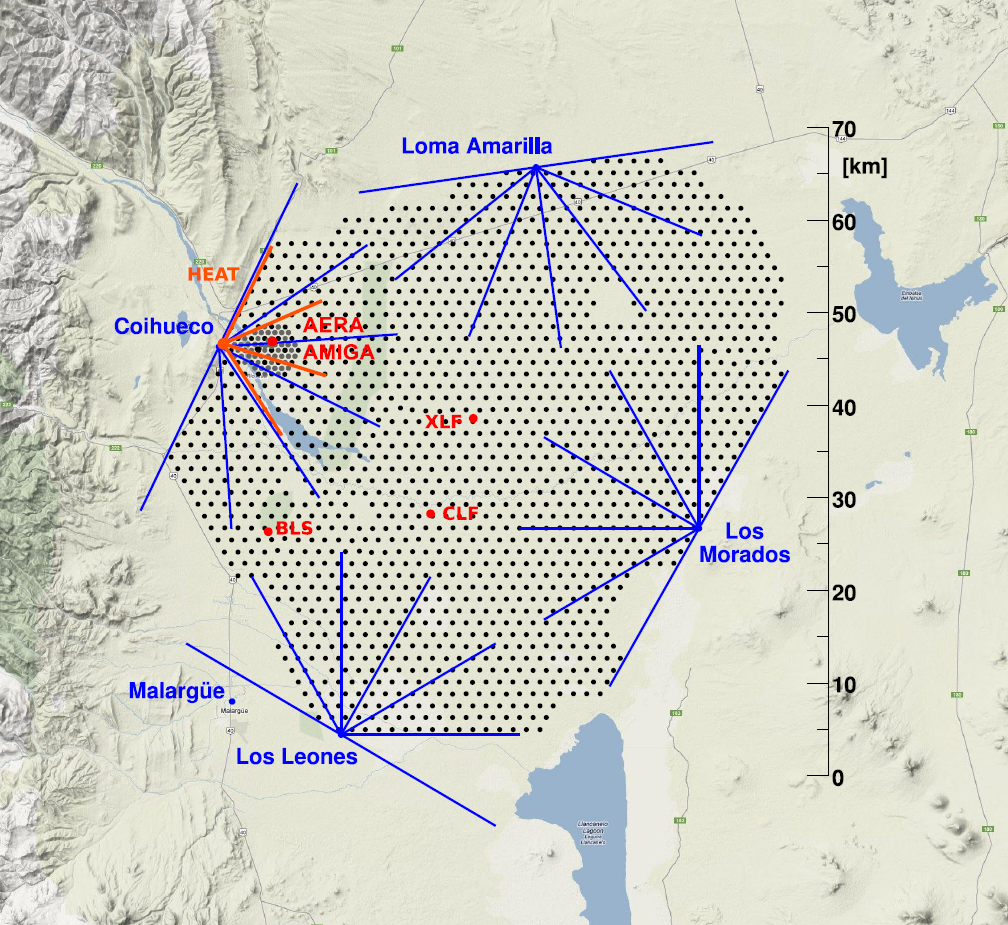
\includegraphics[width=0.98\linewidth]{tesis/mapa_auger.png}
    \column{0.57\textwidth}
      \small
      \begin{itemize}\footnotesize
        \item Propuesto por J.~Cronin y A.~Watson (1991--92) para resolver la
          controversia sobre la supresión.
        \item Construcción 2002--2008; datos desde 2004.
        \item \textbf{1660 tanques} cada 1500\,m ($\approx$3000\,km$^2$) y
          \textbf{27 telescopios} de fluorescencia en 4 sitios.
        \item Arreglos densos (750 y 433\,m) para energías menores: allí está
          \textbf{AMIGA}.
        \item $\sim$400 científicos de 17 países.
      \end{itemize}
      \vspace{3pt}
      \begin{clave}
        Argentina es el país sede. Grupos argentinos ---entre ellos ITeDA---
        diseñan, construyen y operan detectores y analizan los datos.
      \end{clave}
  \end{columns}
  \credito{Mapa: Botti (2019)}
\end{frame}

% ---------------------------------------------------------------- 27
\begin{frame}{Lluvias atmosféricas extensas}
  \begin{columns}[c,onlytextwidth]
    \column{0.42\textwidth}
      \centering
      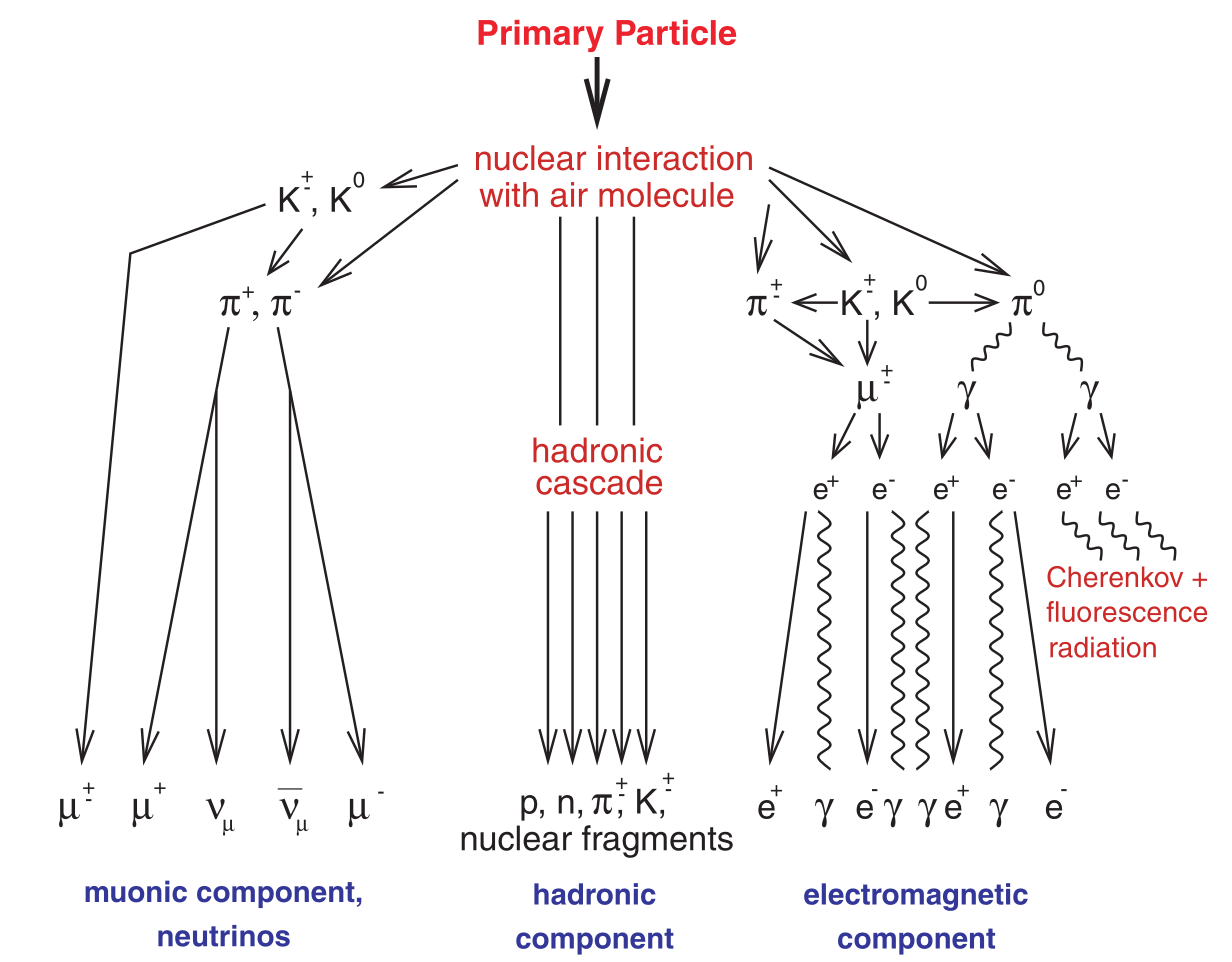
\includegraphics[height=4.1cm]{tesis/eas.png}\\[2pt]
      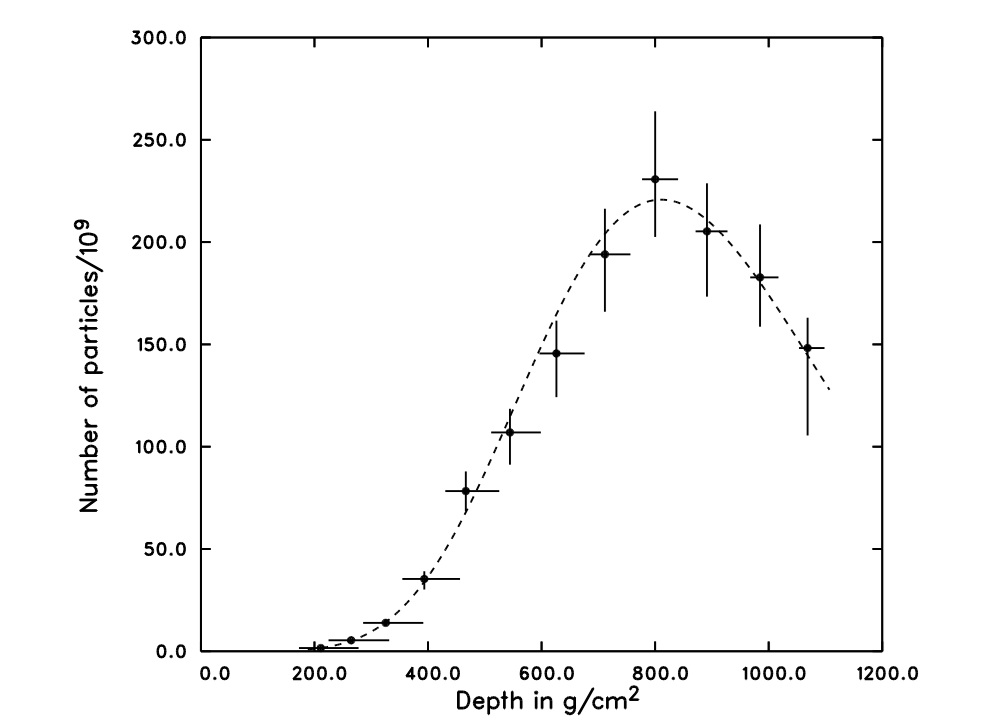
\includegraphics[height=1.9cm]{tesis/ammount_xmax.jpg}\\
      {\tiny Perfil del evento de Fly's Eye ($3{,}2\times10^{20}$\,eV)}
    \column{0.55\textwidth}
      \small
      Primera interacción a $\sim$15--20\,km de altura:
      \begin{itemize}\footnotesize
        \item $\pi^0\to\gamma\gamma$: componente \textbf{electromagnética},
          $\sim$90\% de la energía.
        \item $\pi^\pm\to\mu^\pm\nu_\mu$: componente \textbf{muónica}, penetrante.
      \end{itemize}
      Heitler--Matthews: un núcleo $A$ son $A$ nucleones de energía $E/A$.
      \[ \langle X_\mathrm{max}\rangle \simeq X_0^p + D_{10}\log_{10}\frac{E}{A},
         \quad N_\mu \simeq A\left(\frac{E/A}{\xi_c^\pi}\right)^{\!\beta} \]
      \begin{clave}
        Con $\beta\approx0{,}9$: el hierro tiene $\sim$1,5 veces más muones y llega
        a su máximo $\sim$100\,g/cm$^2$ antes que un protón.
      \end{clave}
  \end{columns}
  \credito{Esquema: Haungs \textit{et al.} (2003). Perfil: Bird \textit{et al.}, ApJ 441 (1995) 144}
\end{frame}

% ---------------------------------------------------------------- 28
\begin{frame}{Detección híbrida: el suelo y el cielo}
  \begin{columns}[T,onlytextwidth]
    \column{0.31\textwidth}
      \centering
      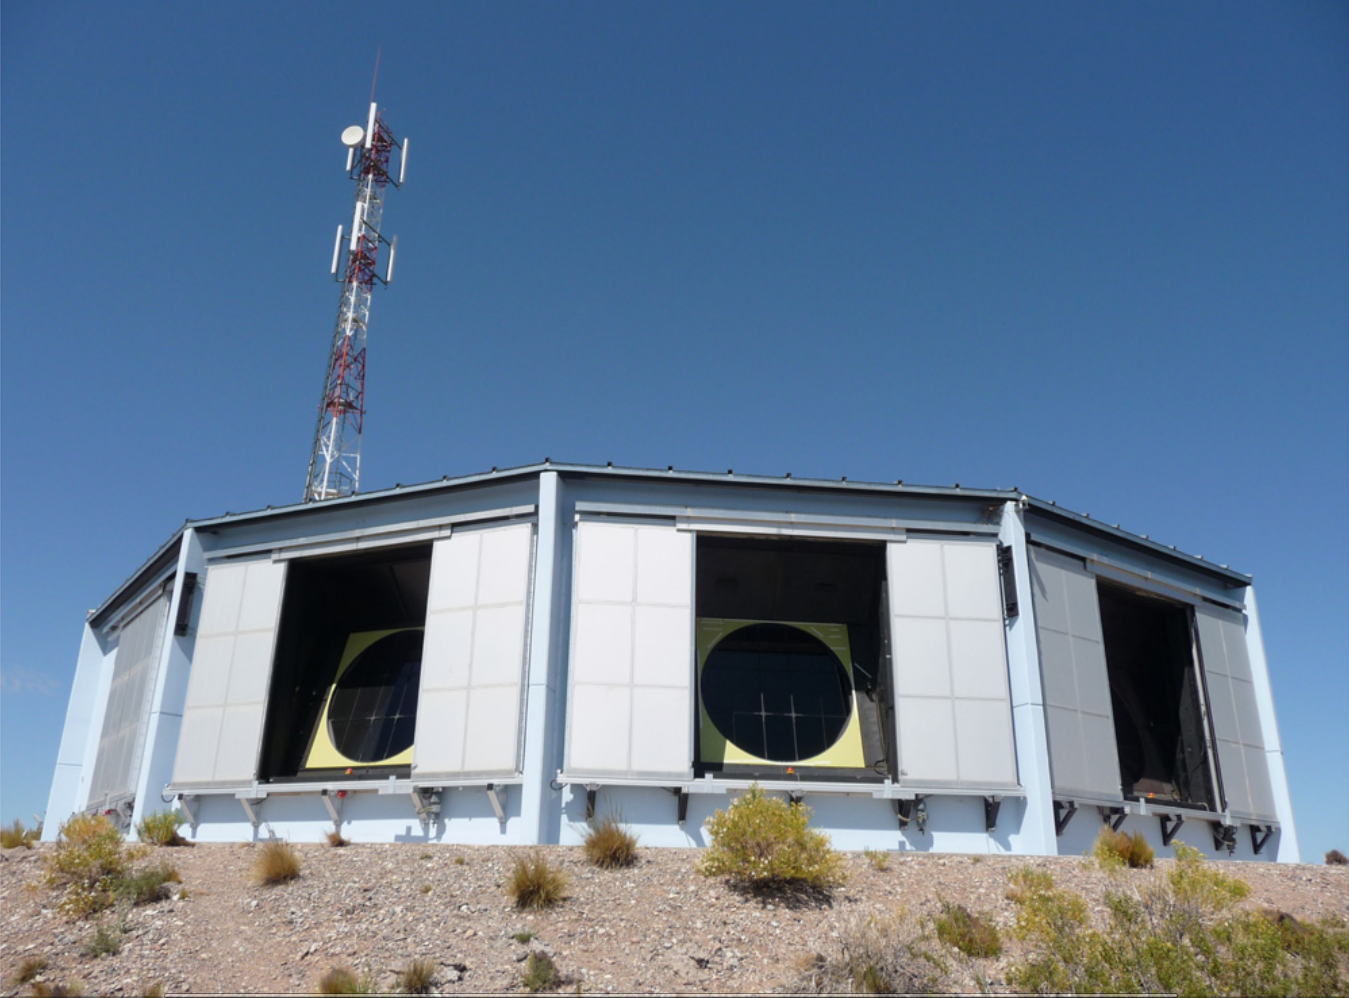
\includegraphics[width=\linewidth]{tesis/fd_leones.png}\\[2pt]
      {\small\bfseries Fluorescencia (FD)}\\[1pt]
      {\footnotesize El N$_2$ excitado emite UV: se \textbf{ve la lluvia
      crecer}. Sólo en noches oscuras ($\sim$15\%).}
    \column{0.31\textwidth}
      \centering
      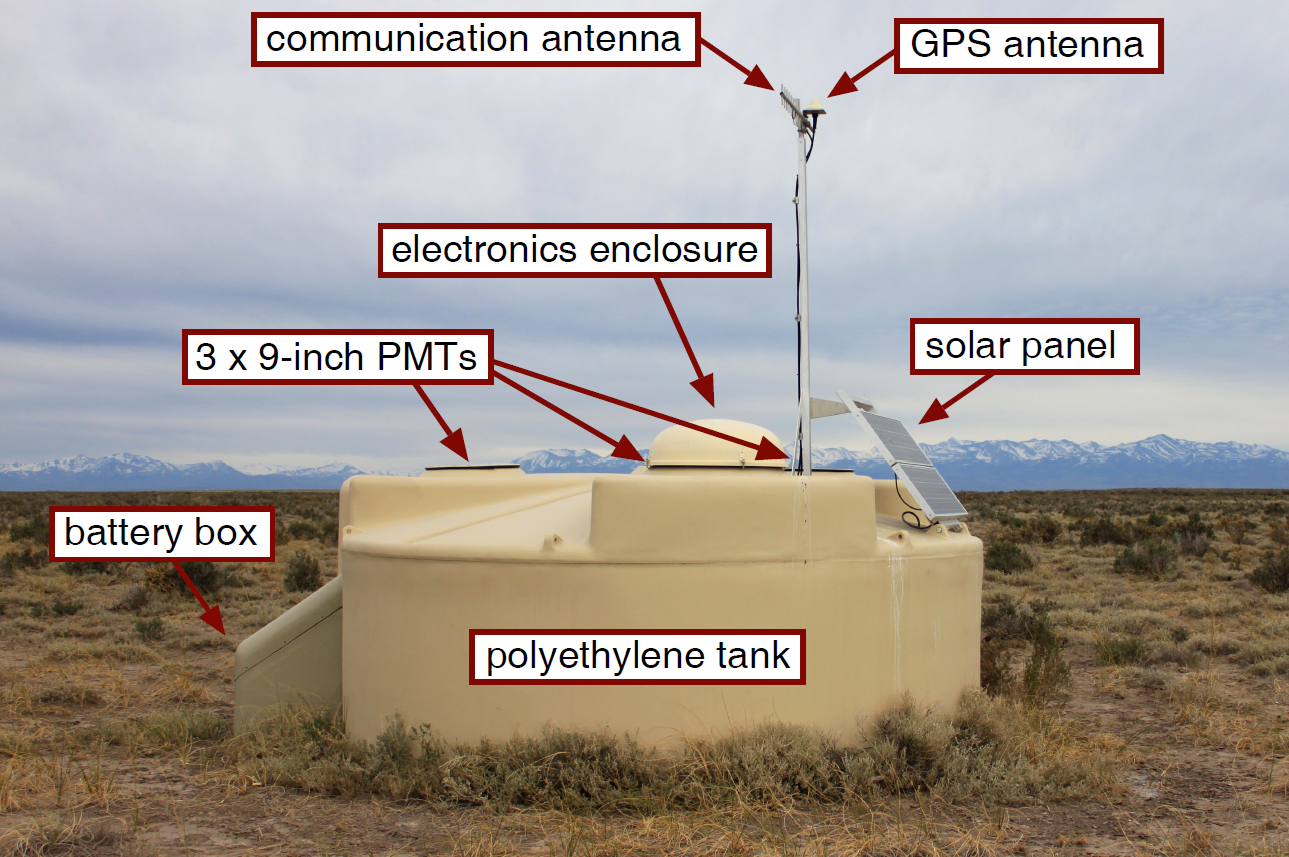
\includegraphics[width=\linewidth]{tesis/ssd.png}\\[2pt]
      {\small\bfseries Superficie (SD)}\\[1pt]
      {\footnotesize 12.000\,l de agua ultrapura y 3 PMT muestrean las
      partículas en el suelo, \textbf{día y noche}.}
    \column{0.33\textwidth}
      \centering
      \begin{tikzpicture}[x=1cm,y=1cm]
        \tikzset{caja/.style={rounded corners=2pt, inner sep=3pt,
          font=\footnotesize, text width=4.1cm, align=left}}
        \node[caja, fill=itedaOrange!15] (a) at (0,2.1)
          {\textbf{FD}: perfil $dE/dX$ $\to$ energía y $X_\mathrm{max}$};
        \node[caja, fill=itedaTeal!15] (b) at (0,0.7)
          {\textbf{SD}: densidad lateral $\to$ $S(1000)$ y dirección};
        \draw[flecha, itedaTealDark] (a.south) -- (b.north)
          node[midway, right, font=\tiny] {calibra};
      \end{tikzpicture}\\[6pt]
      \begin{clave}
        Los eventos \textbf{híbridos} calibran la energía del SD sin
        depender de simulaciones: escala con $\sim$14\% de sistemático.
      \end{clave}
  \end{columns}
  \credito{Fotos: Colaboración Pierre Auger, NIM A 798 (2015); Botti (2019)}
\end{frame}

% ---------------------------------------------------------------- 29
\begin{frame}{AugerPrime y AMIGA: separar electrones de muones}
  \begin{columns}[c,onlytextwidth]
    \column{0.35\textwidth}
      \centering
      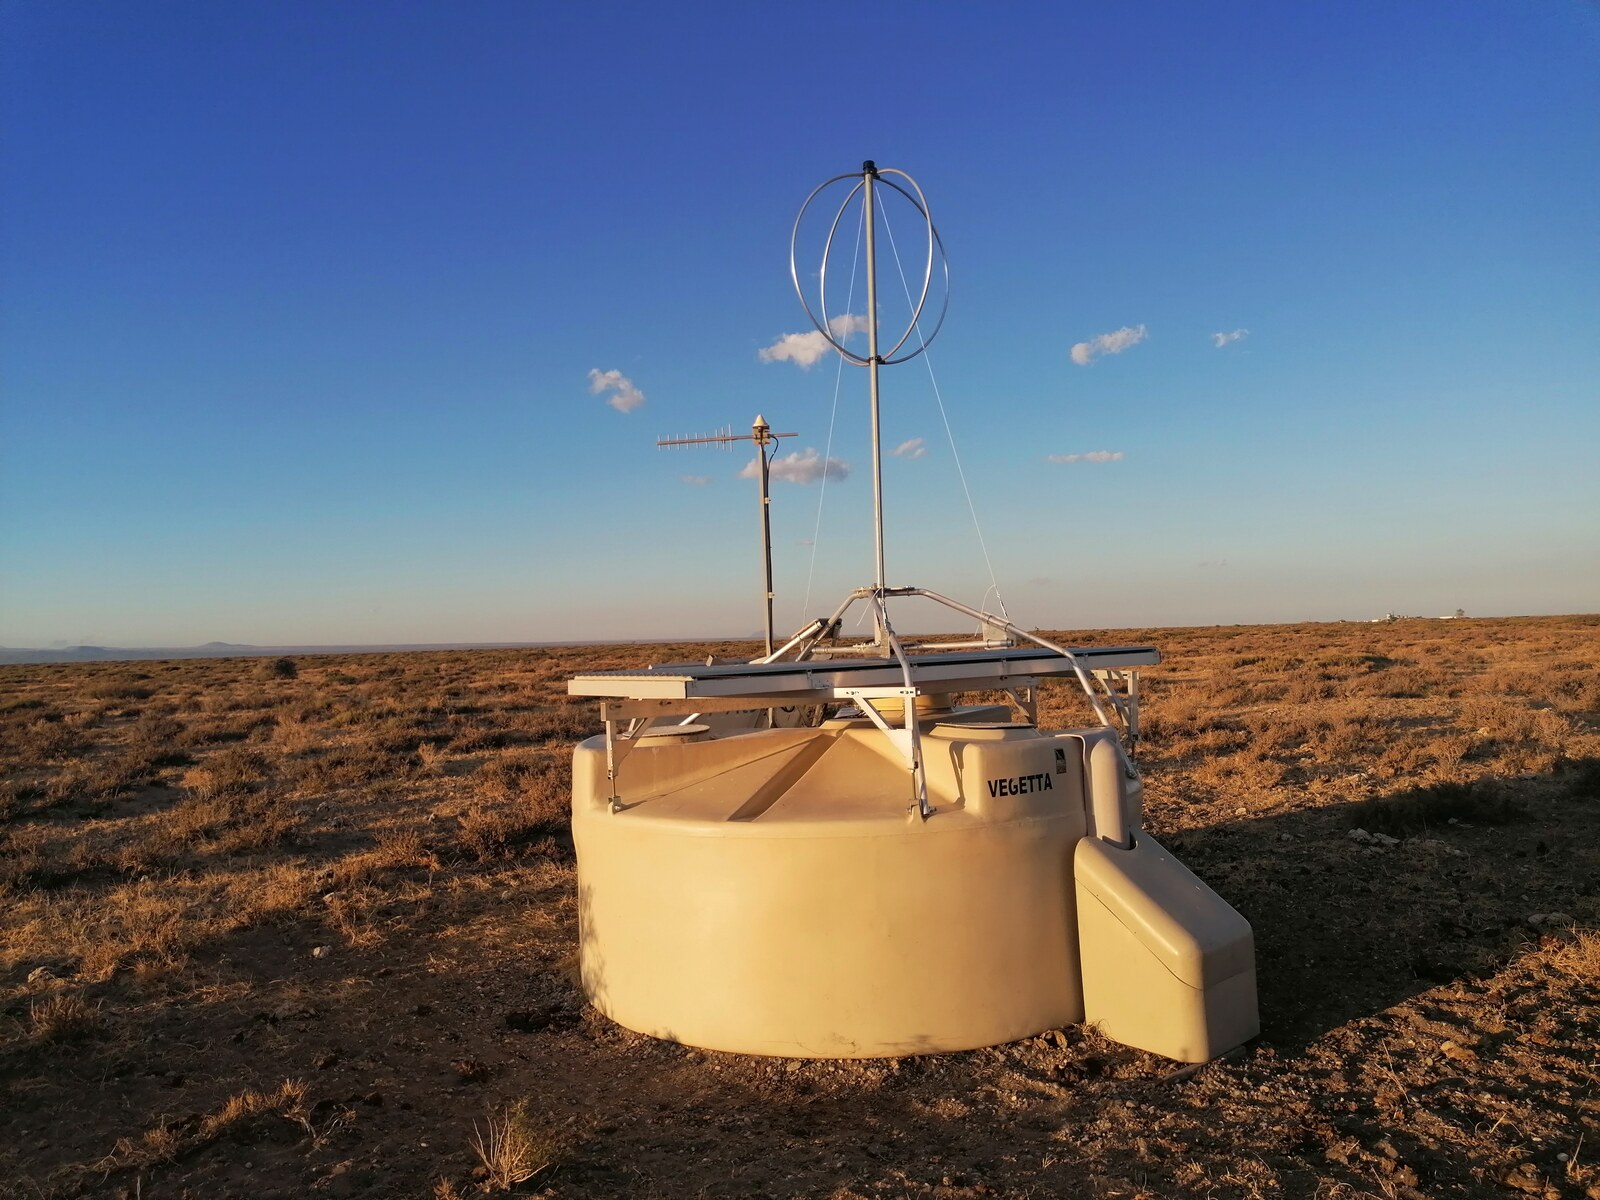
\includegraphics[width=\linewidth]{tesis/estacion_augerprime.jpg}\\[1pt]
      {\scriptsize Estación de AugerPrime}
    \column{0.30\textwidth}
      \begin{itemize}\footnotesize
        \item \textbf{SSD}: centellador de 3,8\,m$^2$ sobre el tanque.
        \item \textbf{RD}: antena de radio, 30--80\,MHz.
        \item \textbf{UMD}: muones \textbf{bajo tierra}.
      \end{itemize}
    \column{0.31\textwidth}
      \centering
      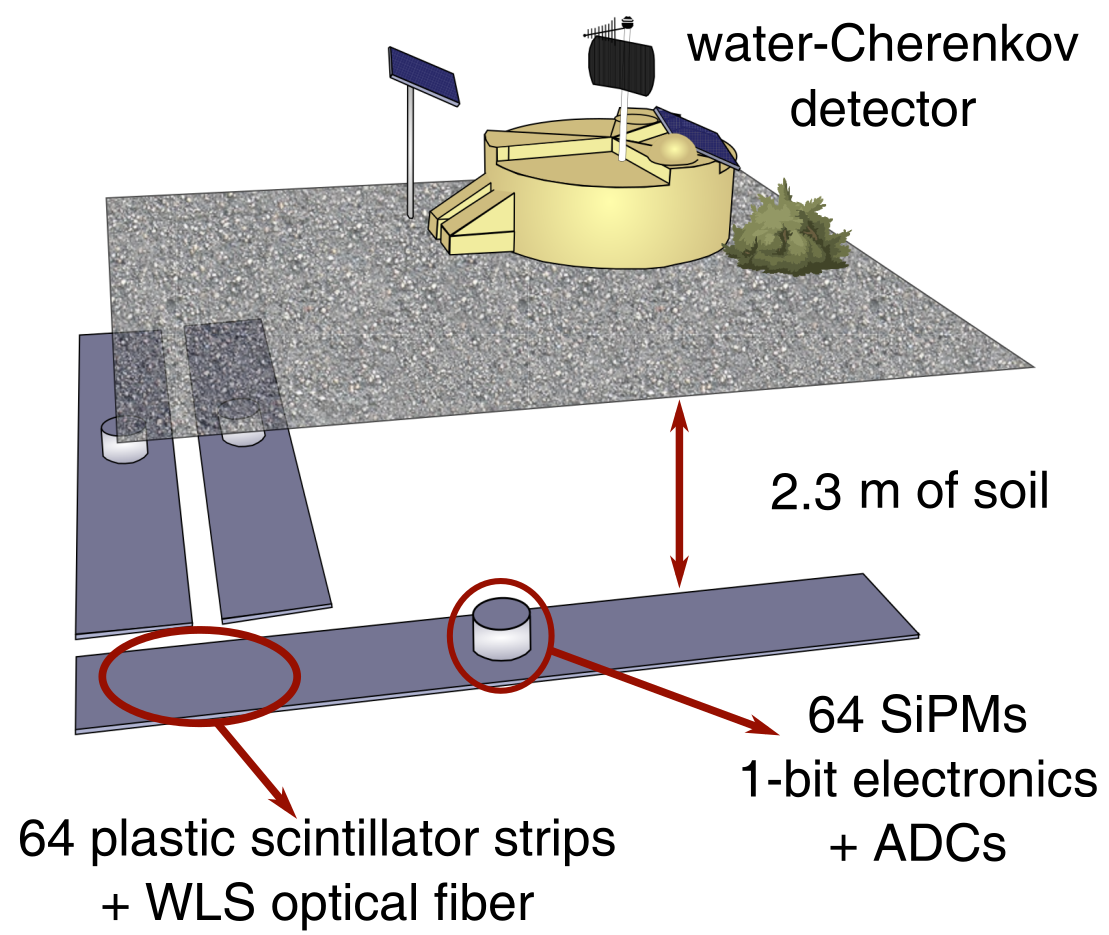
\includegraphics[width=\linewidth]{tesis/umd.png}\\[1pt]
      {\scriptsize AMIGA: módulos enterrados junto a los tanques}
  \end{columns}
  \vspace{8pt}
  \begin{clave}
    Tanque + centellador separan las componentes \textbf{estadísticamente};
    el UMD las separa \textbf{físicamente}: la tierra absorbe lo electromagnético.
  \end{clave}
  \credito{Foto: Colaboración Pierre Auger. Esquema: Botti (2019)}
\end{frame}

% ---------------------------------------------------------------- 30
\begin{frame}{El efecto Cherenkov: una onda de choque de luz}
  \begin{columns}[T,onlytextwidth]
    \column{0.30\textwidth}
      \centering
      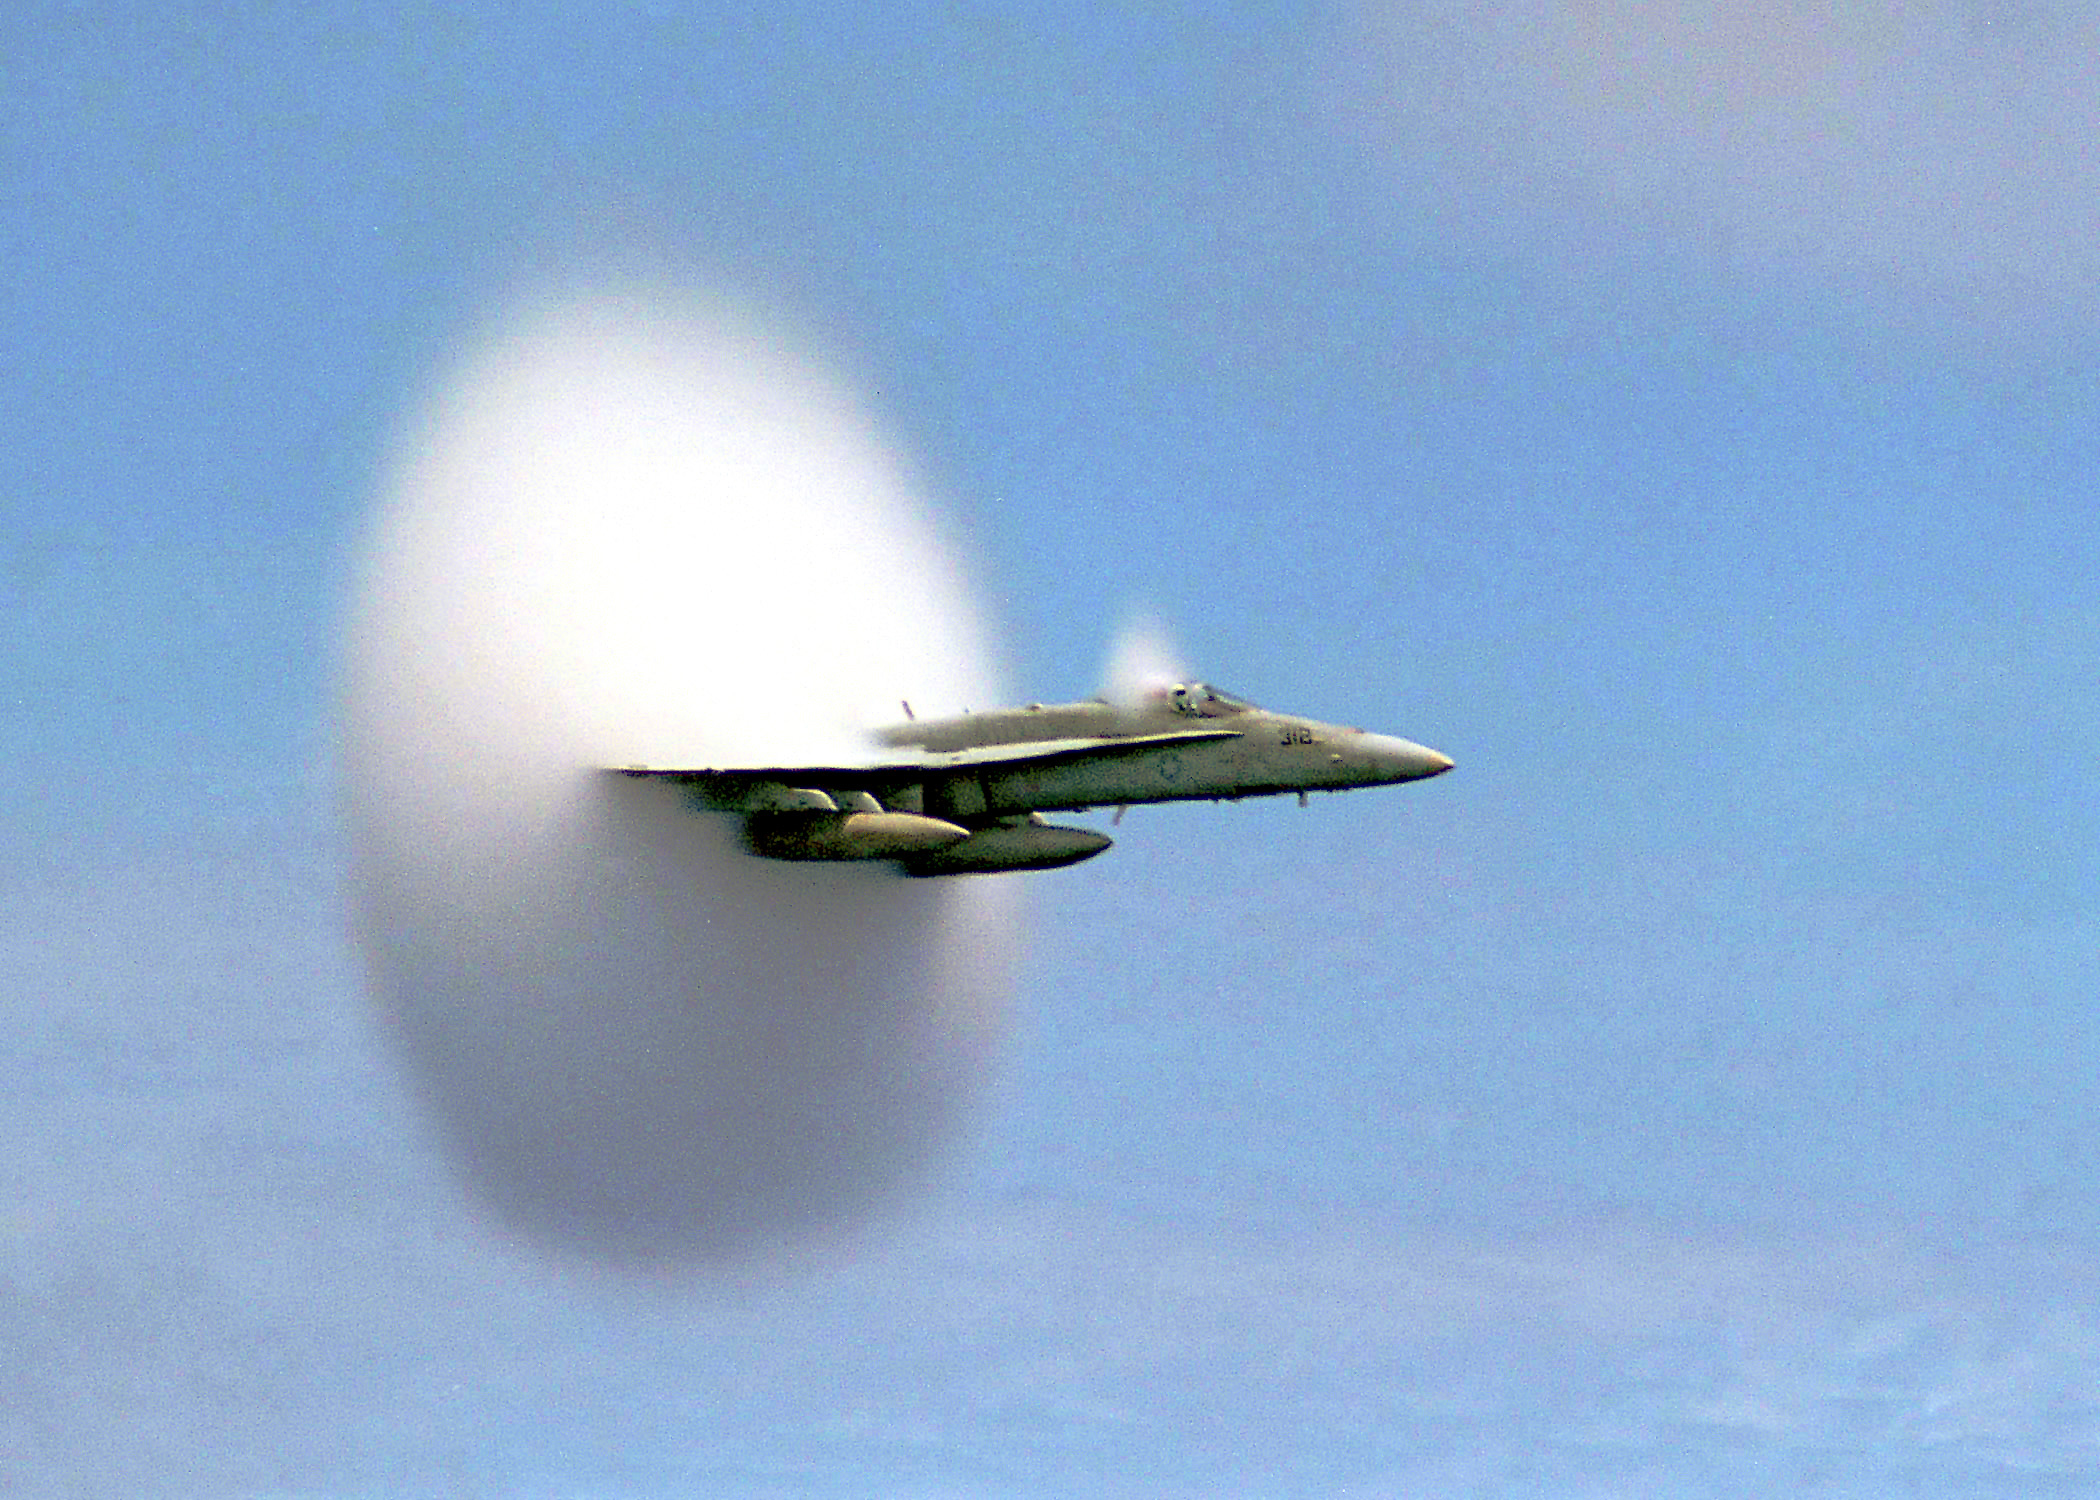
\includegraphics[width=\linewidth]{externas/fa18_cono_vapor.jpg}\\[3pt]
      \begin{tikzpicture}[x=0.42cm,y=0.42cm]
        \begin{scope}
          \clip (-4.6,-2.3) rectangle (1.6,2.3);
          \foreach \i in {0,...,4}{
            \pgfmathsetmacro{\xx}{-4+\i}\pgfmathsetmacro{\rr}{0.6*(5-\i)}
            \draw[itedaGray] (\xx,0) circle (\rr);}
          \draw[itedaOrange, thick] (1,0) -- ++(143.1:4.2);
          \draw[itedaOrange, thick] (1,0) -- ++(216.9:4.2);
        \end{scope}
        \fill[itedaTealDark] (1,0) circle (2.2pt);
      \end{tikzpicture}\\[1pt]
      {\footnotesize Sonido: $\sin\alpha = v_s/v$}
    \column{0.36\textwidth}
      \centering
      \begin{tikzpicture}[x=0.62cm,y=0.62cm]
        \begin{scope}
          \clip (-4.6,-2.75) rectangle (1.7,2.75);
          \fill[hielo!18] (-4.6,-2.75) rectangle (1.7,2.75);
          \foreach \i in {0,...,4}{
            \pgfmathsetmacro{\xx}{-4+\i}\pgfmathsetmacro{\rr}{0.752*(5-\i)}
            \draw[cmbAzul!70] (\xx,0) circle (\rr);
            \fill[cmbAzul] (\xx,0) circle (1pt);}
          \draw[itedaOrange, very thick] (1,0) -- ++(131.2:3.6);
          \draw[itedaOrange, very thick] (1,0) -- ++(228.8:3.6);
        \end{scope}
        \draw[flecha, itedaTealDark] (-4.5,0) -- (1.6,0);
        \fill[itedaTealDark] (1,0) circle (2.5pt);
        \draw[-{Stealth}, itedaOrange, very thick] (-0.05,1.2) -- ++(41.2:1.3);
        \draw[-{Stealth}, itedaOrange, very thick] (-0.05,-1.2) -- ++(-41.2:1.3);
        \draw[dashed, itedaGray] (-0.05,1.2) -- ++(1.2,0);
        \draw[itedaGray] (0.55,1.2) arc (0:41.2:0.6);
        \node[font=\scriptsize] at (0.95,1.45) {$\theta_C$};
        \node[font=\scriptsize, anchor=north west] at (-4.5,-0.1) {$\beta c > c/n$};
      \end{tikzpicture}\\[1pt]
      \small
      \[ \cos\theta_C=\frac{1}{\beta n} \]
      {\footnotesize Agua: $n=1{,}33$, $c/n=2{,}25\times10^{8}$\,m/s,
      $\theta_C\le 41^\circ$.}
    \column{0.30\textwidth}
      \centering
      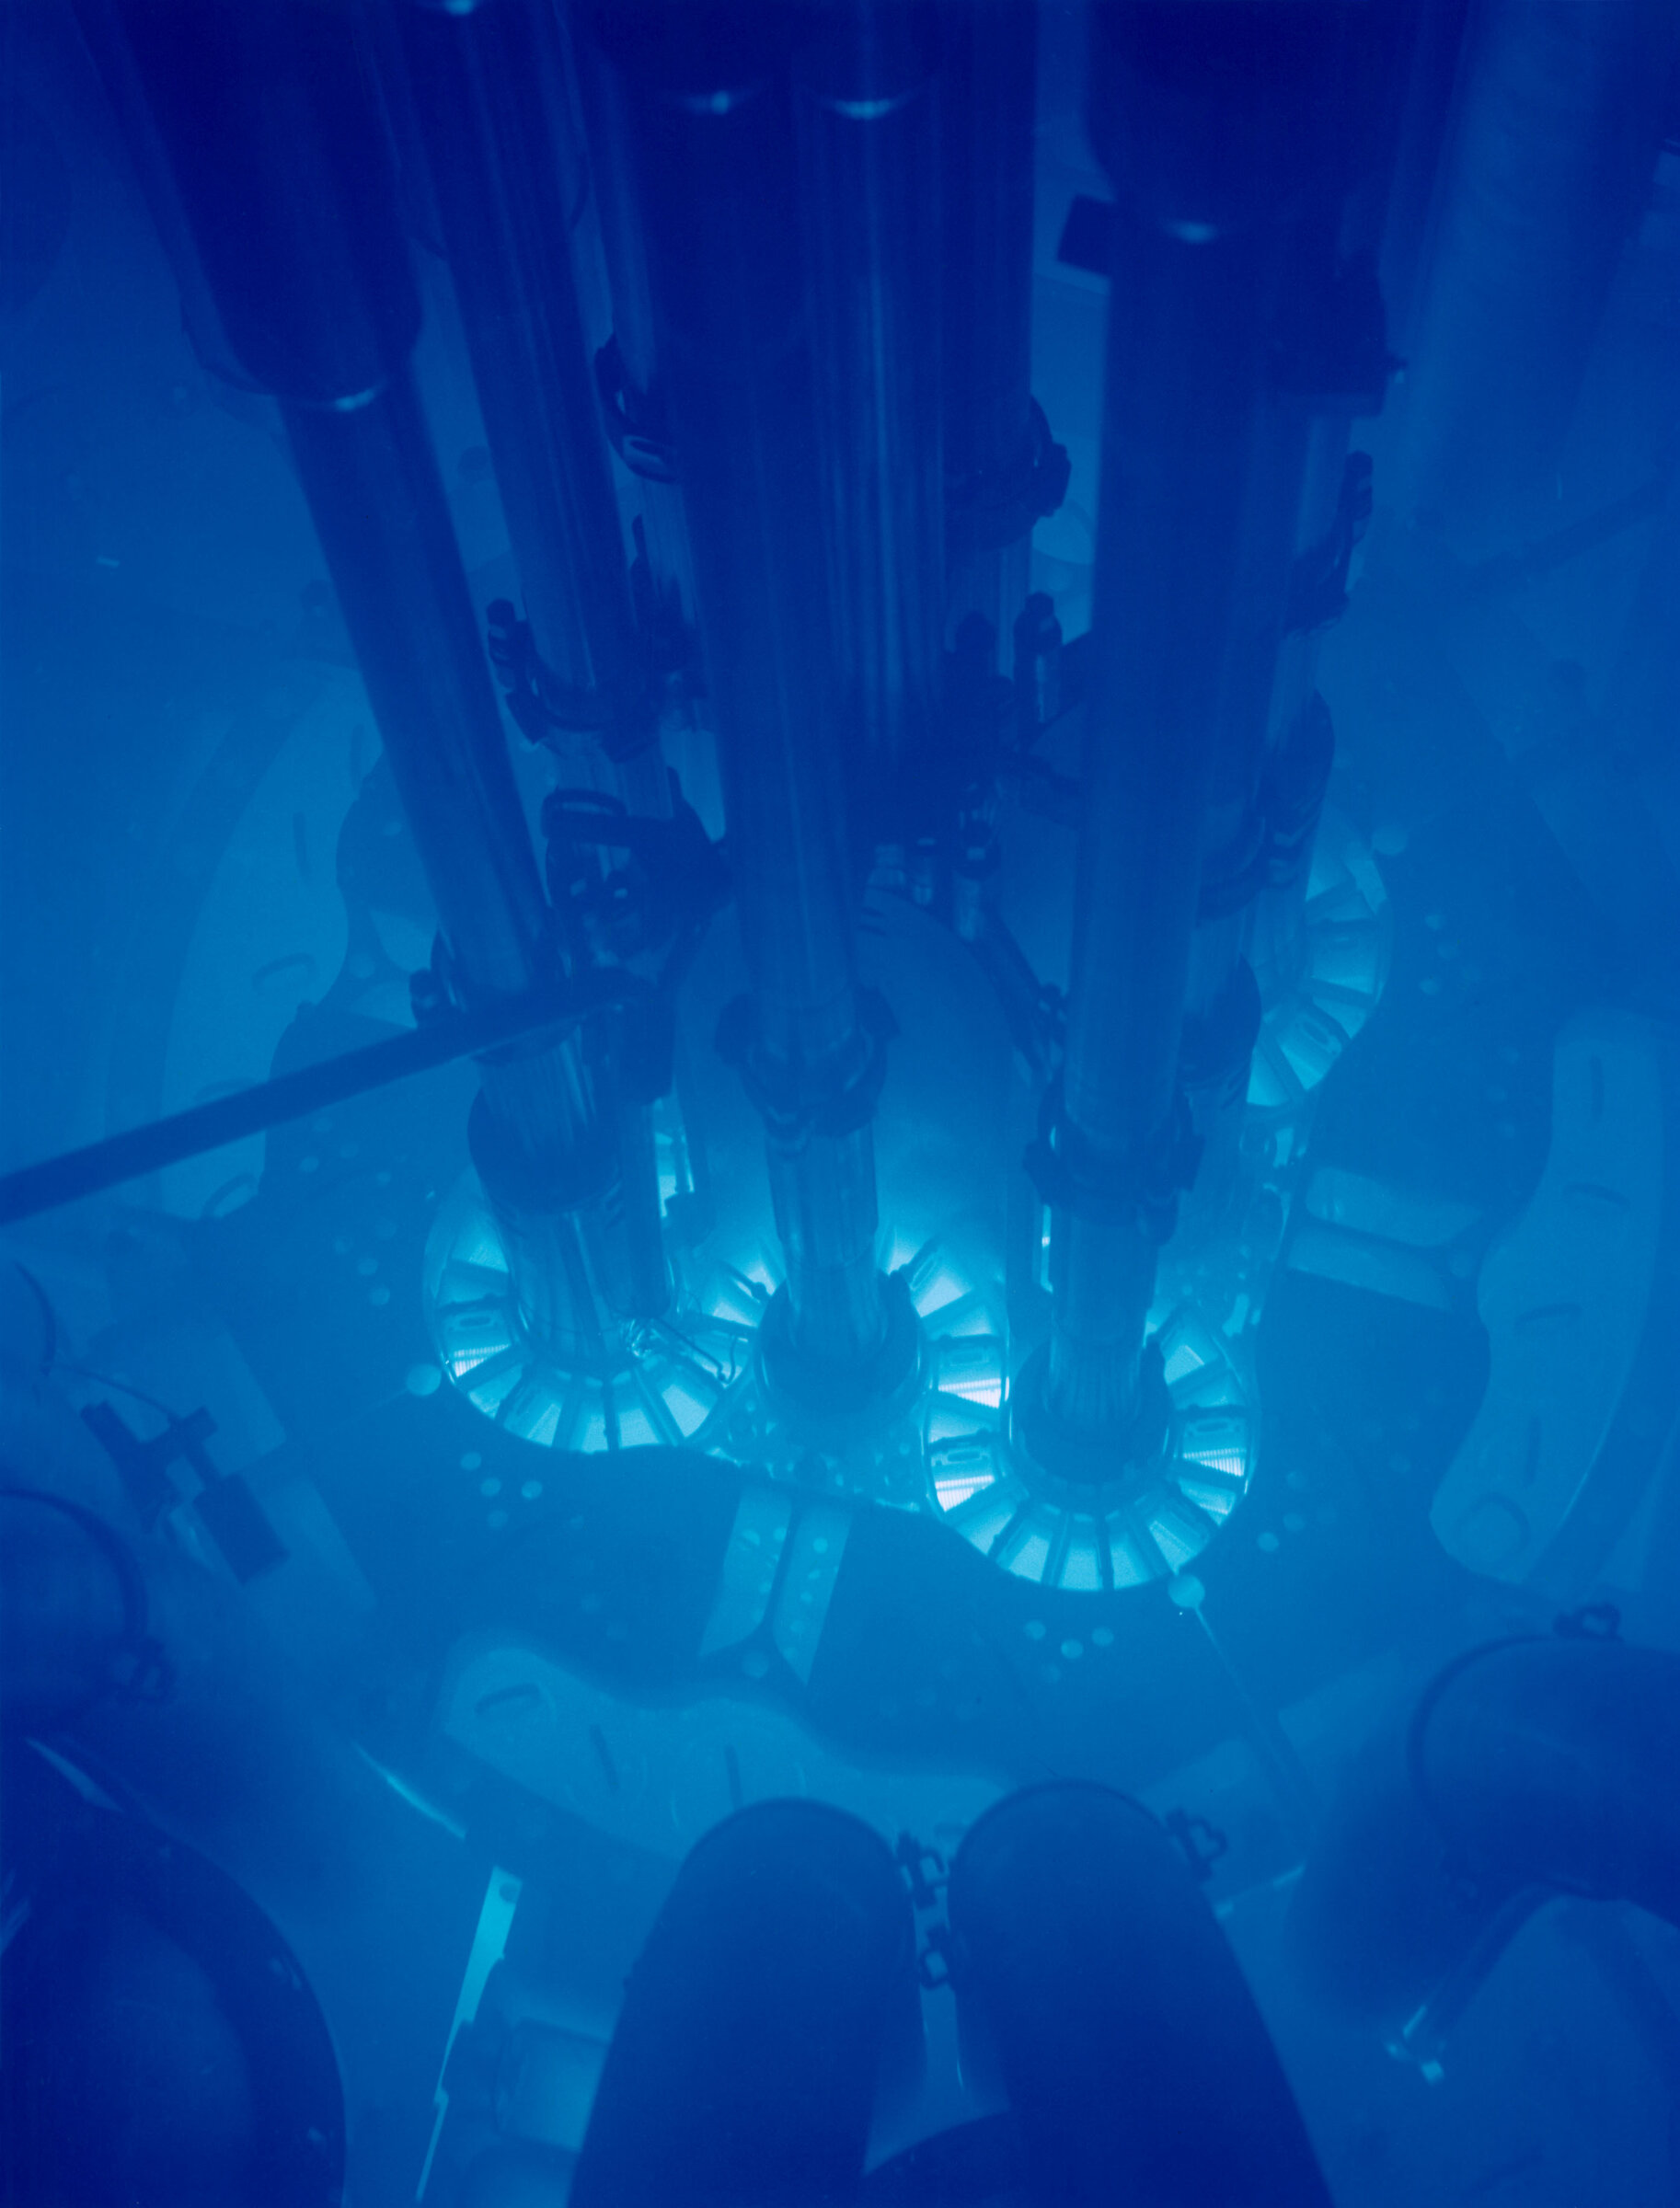
\includegraphics[height=2.1cm]{externas/cherenkov_reactor_ATR.jpg}\\[1pt]
      {\scriptsize Brillo Cherenkov en un reactor}\\[4pt]
      \begin{clave}
        Para emitir hay que ir más rápido que la luz en el agua
        ($\beta>0{,}75$): un electrón necesita \textbf{0,26\,MeV}, un muón
        \textbf{54\,MeV}. Luego emite $\sim$300 fotones/cm.
      \end{clave}
  \end{columns}
  \creditoizq{Fotos: US Navy (dom.\ público); Argonne Natl.\ Lab., CC BY-SA 2.0}
\end{frame}

% ---------------------------------------------------------------- 31
\begin{frame}{Qué medimos realmente: trazas, tiempos y una función lateral}
  \begin{columns}[c,onlytextwidth]
    \column{0.46\textwidth}
      \centering
      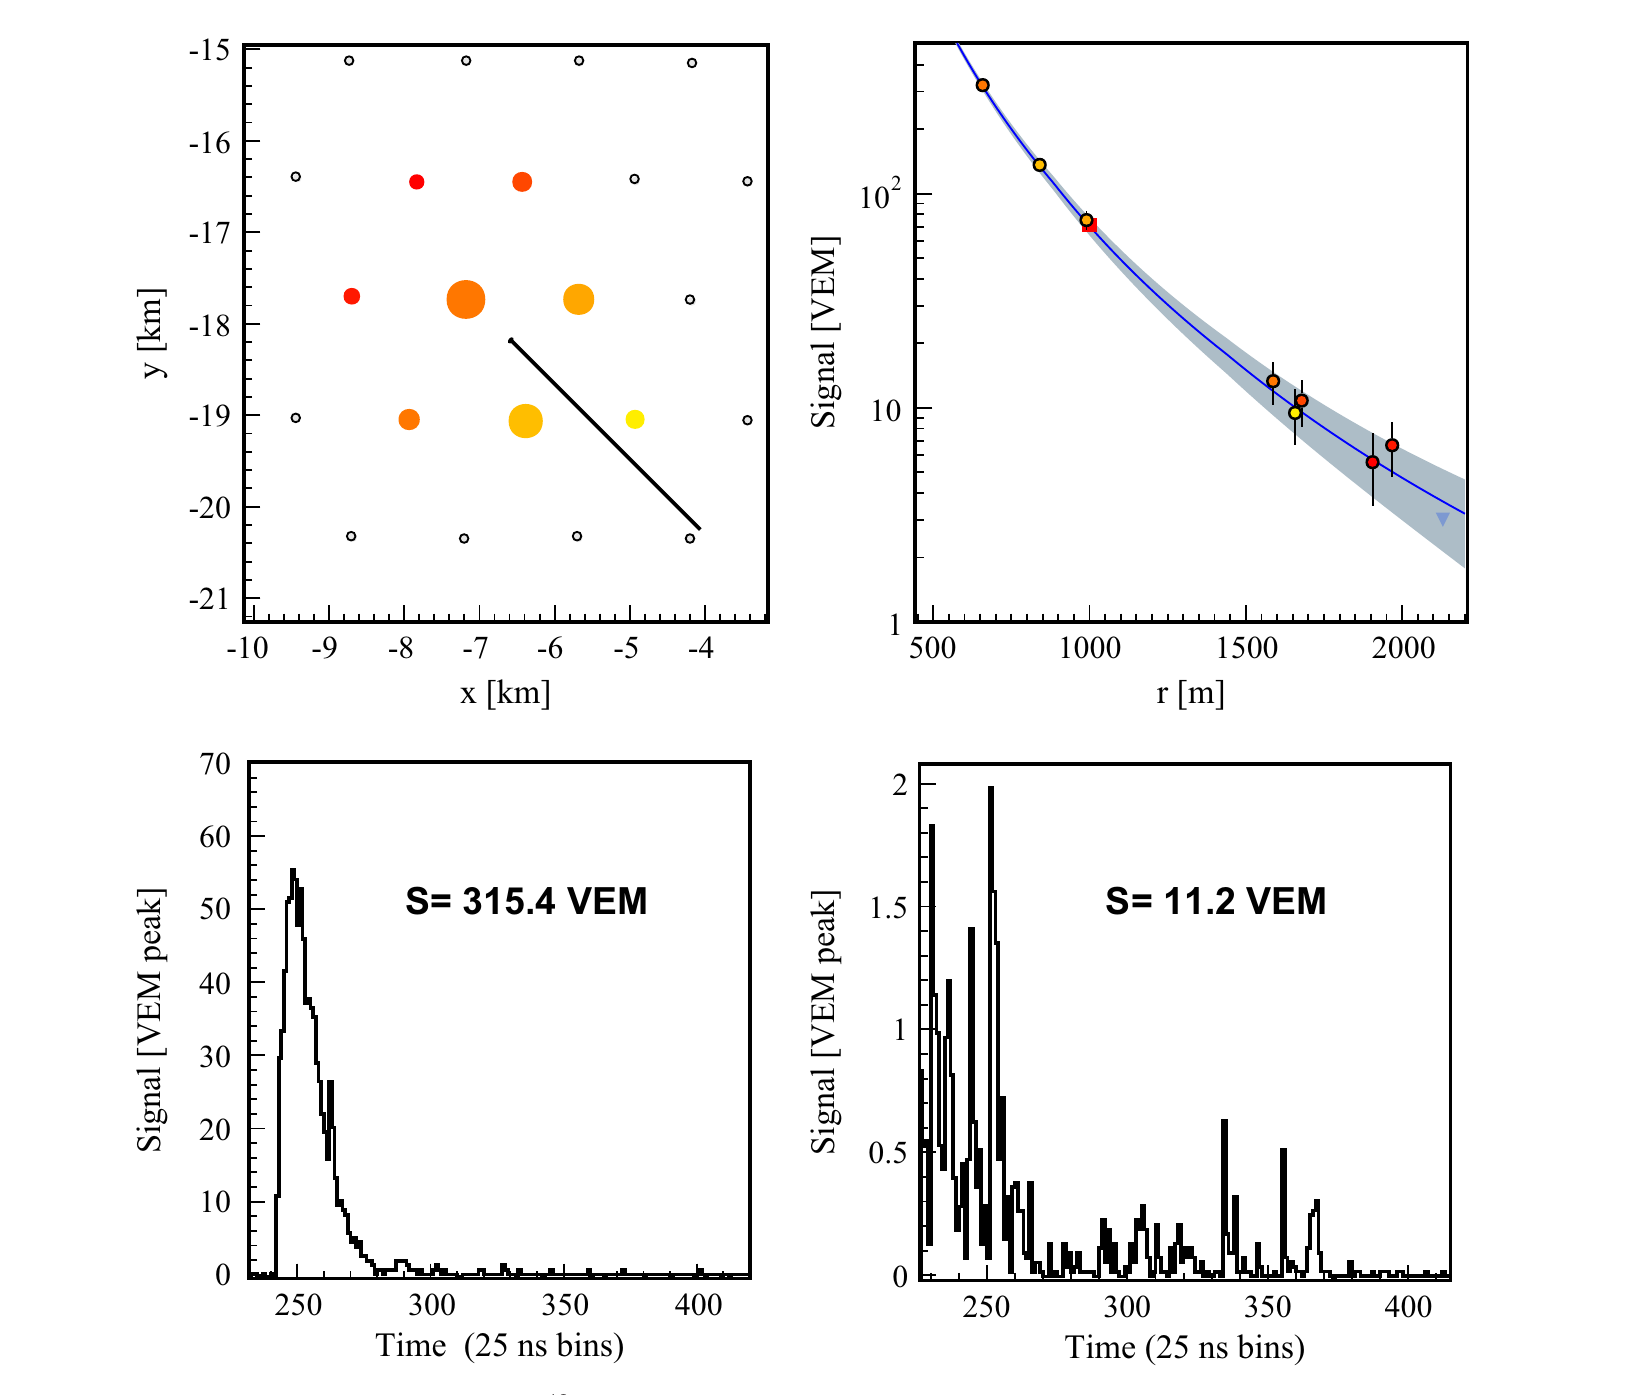
\includegraphics[width=\linewidth]{externas/auger_sd_evento_trazas.png}
    \column{0.51\textwidth}
      \small
      Evento de $\sim3\times10^{19}$\,eV, $\theta=28^\circ$, 8 estaciones.
      \begin{enumerate}\footnotesize
        \item \textbf{Trazas} cada 25\,ns, en \textbf{VEM}: cerca del núcleo un
          pulso grande; lejos, muones aislados.
        \item \textbf{Tiempos} de arribo $\to$ frente de la lluvia $\to$
          dirección ($\sim$1$^\circ$).
        \item \textbf{Señales} $\to$ función lateral $\to$ $S(1000)$ $\to$
          \textbf{energía} (calibrada con el FD).
      \end{enumerate}
      \begin{clave}
        Nunca vemos el primario: \textbf{inferimos} energía, dirección y masa
        desde sus secundarios, con incertezas estadísticas y sistemáticas.
      \end{clave}
  \end{columns}
  \credito{Figura: Colaboración Pierre Auger, NIM A 798 (2015) 172, Fig.~17}
\end{frame}

% ---------------------------------------------------------------- 32
\begin{frame}{Muones: mensajeros de la cascada hadrónica}
  \begin{columns}[c,onlytextwidth]
    \column{0.46\textwidth}
      \centering
      \begin{tikzpicture}[x=1cm,y=0.82cm]
        \draw[itedaGray!50, line width=6pt] (-0.2,-2.65) -- (5.2,-2.65);
        \node[font=\tiny, text=itedaGray, anchor=north west] at (-0.2,-2.75) {suelo};
        \node[font=\small] (h) at (0.4,1.8) {$\pi^\pm$};
        \draw[flecha, itedaTealDark] (0,2.6) -- (h);
        \node[font=\tiny, text=itedaGray, anchor=east] at (0,2.5) {cascada};
        \draw[flecha, itedaOrange, very thick] (h) -- (3.9,-2.55) node[pos=0.55, right, font=\small] {$\mu^\pm$};
        \draw[flecha, violetaNu, dashed] (h) -- (2.4,1.4) node[right, font=\small] {$\nu_\mu$};
        \node[font=\scriptsize, align=left, anchor=west] at (2.6,0.4)
          {$c\tau_\pi = 7{,}8$\,m:\\decae o interactúa};
        \node[font=\scriptsize, align=left, anchor=west] at (3.0,-1.2)
          {$\gamma c\tau_\mu\approx 6$\,km\\a 1\,GeV};
      \end{tikzpicture}\\[4pt]
      {\footnotesize La \textbf{dilatación temporal} los deja llegar
      ($c\tau_\mu=659$\,m); pierden $\sim$2\,GeV en el aire y casi no se desvían.}
    \column{0.51\textwidth}
      \small
      \textbf{Por qué importan}
      \begin{itemize}\footnotesize
        \item $N_\mu\propto A^{1-\beta}E^{\beta}$: sensibles a la \textbf{masa}.
        \item Guardan la memoria de la cascada \textbf{hadrónica}: física de
          partículas a $\sqrt{s}\sim100$\,TeV.
      \end{itemize}
      \begin{clave}
        \textbf{El enigma de los muones}: los datos tienen más señal hadrónica
        que las simulaciones, un factor $1{,}33\pm0{,}16$ (EPOS-LHC) a
        $1{,}61\pm0{,}21$ (QGSJet-II-04) a 6--16\,EeV.
      \end{clave}
  \end{columns}
  \credito{Auger, PRL 117 (2016) 192001}
\end{frame}

% ---------------------------------------------------------------- 33
\begin{frame}{El detector subterráneo de muones (UMD)}
  \begin{columns}[c,onlytextwidth]
    \column{0.43\textwidth}
      \centering
      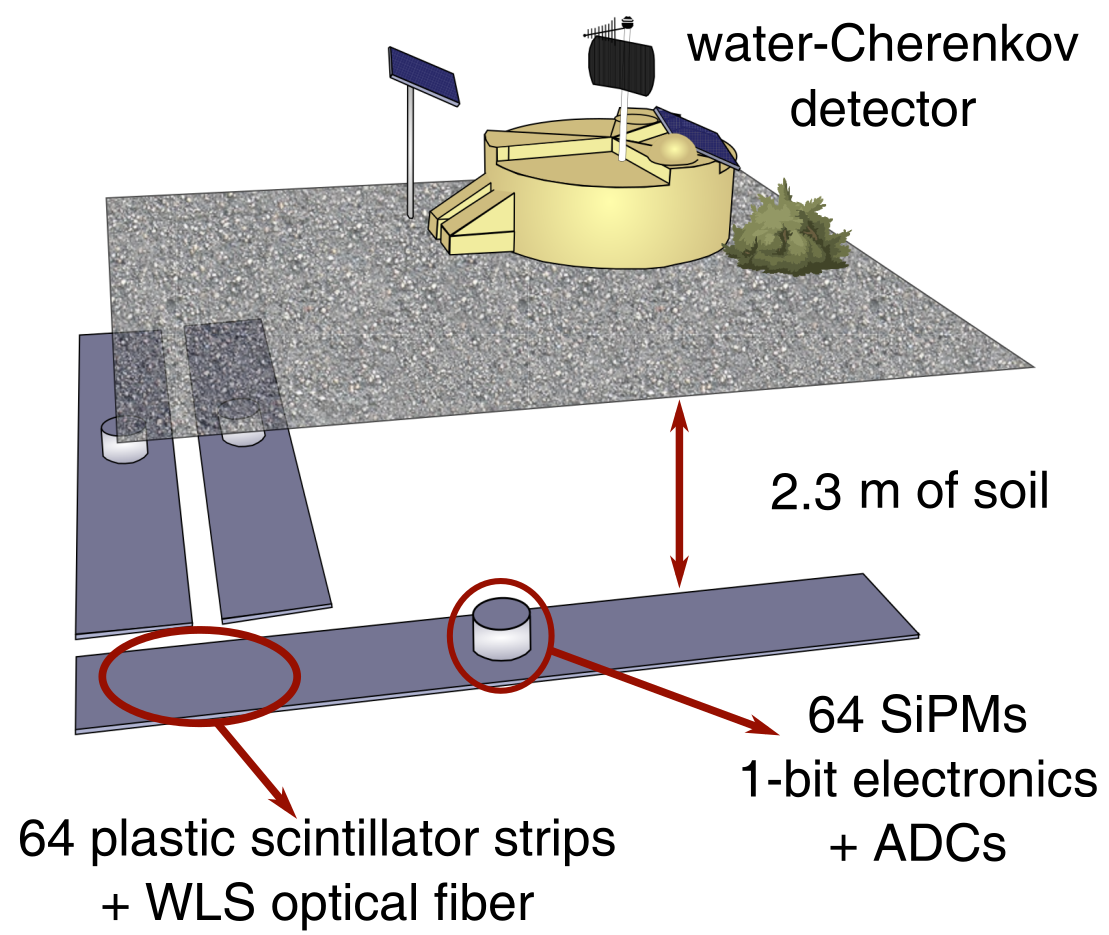
\includegraphics[width=0.82\linewidth]{tesis/umd.png}\\[2pt]
      \begin{itemize}\footnotesize
        \item 3 módulos de 10\,m$^2$ a \textbf{2,3\,m bajo tierra}
          ($\approx$540\,g/cm$^2$): umbral $\sim$1\,GeV$/\cos\theta$.
        \item 64 tiras de \textbf{centellador} por módulo, leídas con SiPMs.
      \end{itemize}
    \column{0.54\textwidth}
      \centering
      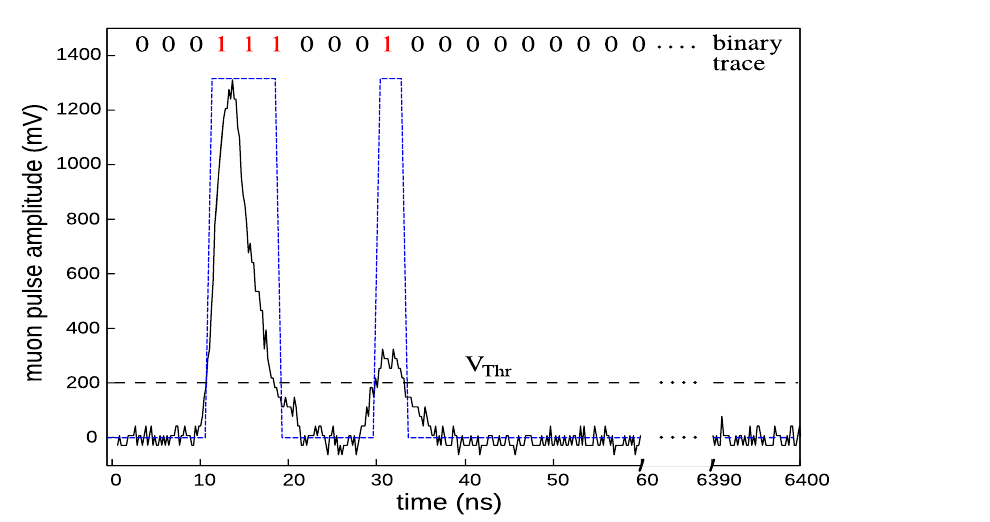
\includegraphics[width=0.85\linewidth]{externas/umd_traza_binaria.png}\\[1pt]
      {\scriptsize Pulso de un muón, discriminado y muestreado cada 3,125\,ns}\\[3pt]
      \begin{clave}
        \textbf{No es Cherenkov}: el muón ioniza y el plástico
        \textbf{centellea}. Cada tira es un contador: un patrón «1x1» es un
        muón y se \textbf{cuentan}. A alta densidad, se integra la carga.
      \end{clave}
  \end{columns}
  \credito{Esquema: Botti (2019). Traza: Colaboración Pierre Auger, EPJC 80 (2020) 751, Fig.~3}
\end{frame}
